\section{Case study : securing legacy code}
\label{sec:case-study}

Securing web application using \textit{Authenticator} security contract

Nous nous sommes intéressés à la mise en oeuvre des patrons de sécurité ou cybercontrats définis dans la bibliothèque de \textit{Patterns} de PAMELA sur un cas d'utilisation représentatif d'une application réelle, l'idée étant de valider l'approche en pratique. 

L'autre élément déterminant de cette expérimentation consistait à valider la pertinence d'une telle approche sur un code existant (\textit{legacy code}), l'idée étant de voir comment sécuriser en aval une application tout à fait fonctionnelle, sans avoir besoin de ré-architecturer tout le code fonctionnel.

Nous nous sommes intéressé à une application Web, et avons choisi le framework Spring\footnote{\url{https://spring.io/}} parce qu'il est d'une part très utilisé et représentatif de l'état de l'art en terme d'ingénierie de sites web, et d'autre part parce que c'est un \textit{framework} codé en Java.

\subsection{Le framework Spring}

\textit{Spring} est un framework de développement d'application Web en java extrêmement populaire.  Ce framework s'appuie sur des librairies prédéfinie comprenant des classes réutilisables. La variété des classes est à la fois un avantage pour offrir au développeur de nombreuses possibilités mais aussi un inconvénient qui implique que Spring est très étendu et long à assimiler au premier abord, ce qui peut poser de nombreux problèmes en terme de sécurité par d'adjonction inopportune de bugs ou de failles de sécurité. Il est surtout reconnu pour son injection de dépendance et pour l’inversion de contrôle. Spring comporte un module web qui supporte l’API Servlet (interface de programmation applicative pour les classes Java qui permettent de créer dynamiquement des données au sein d’un serveur HTTP) qui s’appelle Spring MVC pour Model View Controller.

La figure \ref{fig:ArchitectureSpring} présente d'architecture du framework.
Le \textit{DispatcherServlet} de \textit{Spring} gère toute les requêtes reçues par l’application (1) , il va d’abord solliciter le \textit{HandlerMapping} (2) qui va faire le lien avec un bean contrôleur enregistré annoté par \texttt{@Controller}. Celui-ci va ensuite exécuter la logique d’application fournie par le \textit{HandlerAdapter} qui va résulter en un modèle. Il va aussi retourner un nom logique de vue au \textit{HandlerAdapter} (3) . Après cela, le \textit{DispatcherServlet} va solliciter le \textit{ViewResolver} (4) qui va résoudre la \textit{View} grâce au nom logique (5) . Le \textit{DispatcherServlet} envoie ensuite le processus de rendu à la vue renvoyée qui va constituer avec le modèle la réponse à la requête initialement reçue (6) .

\begin{figure}[!h]
    \centering
    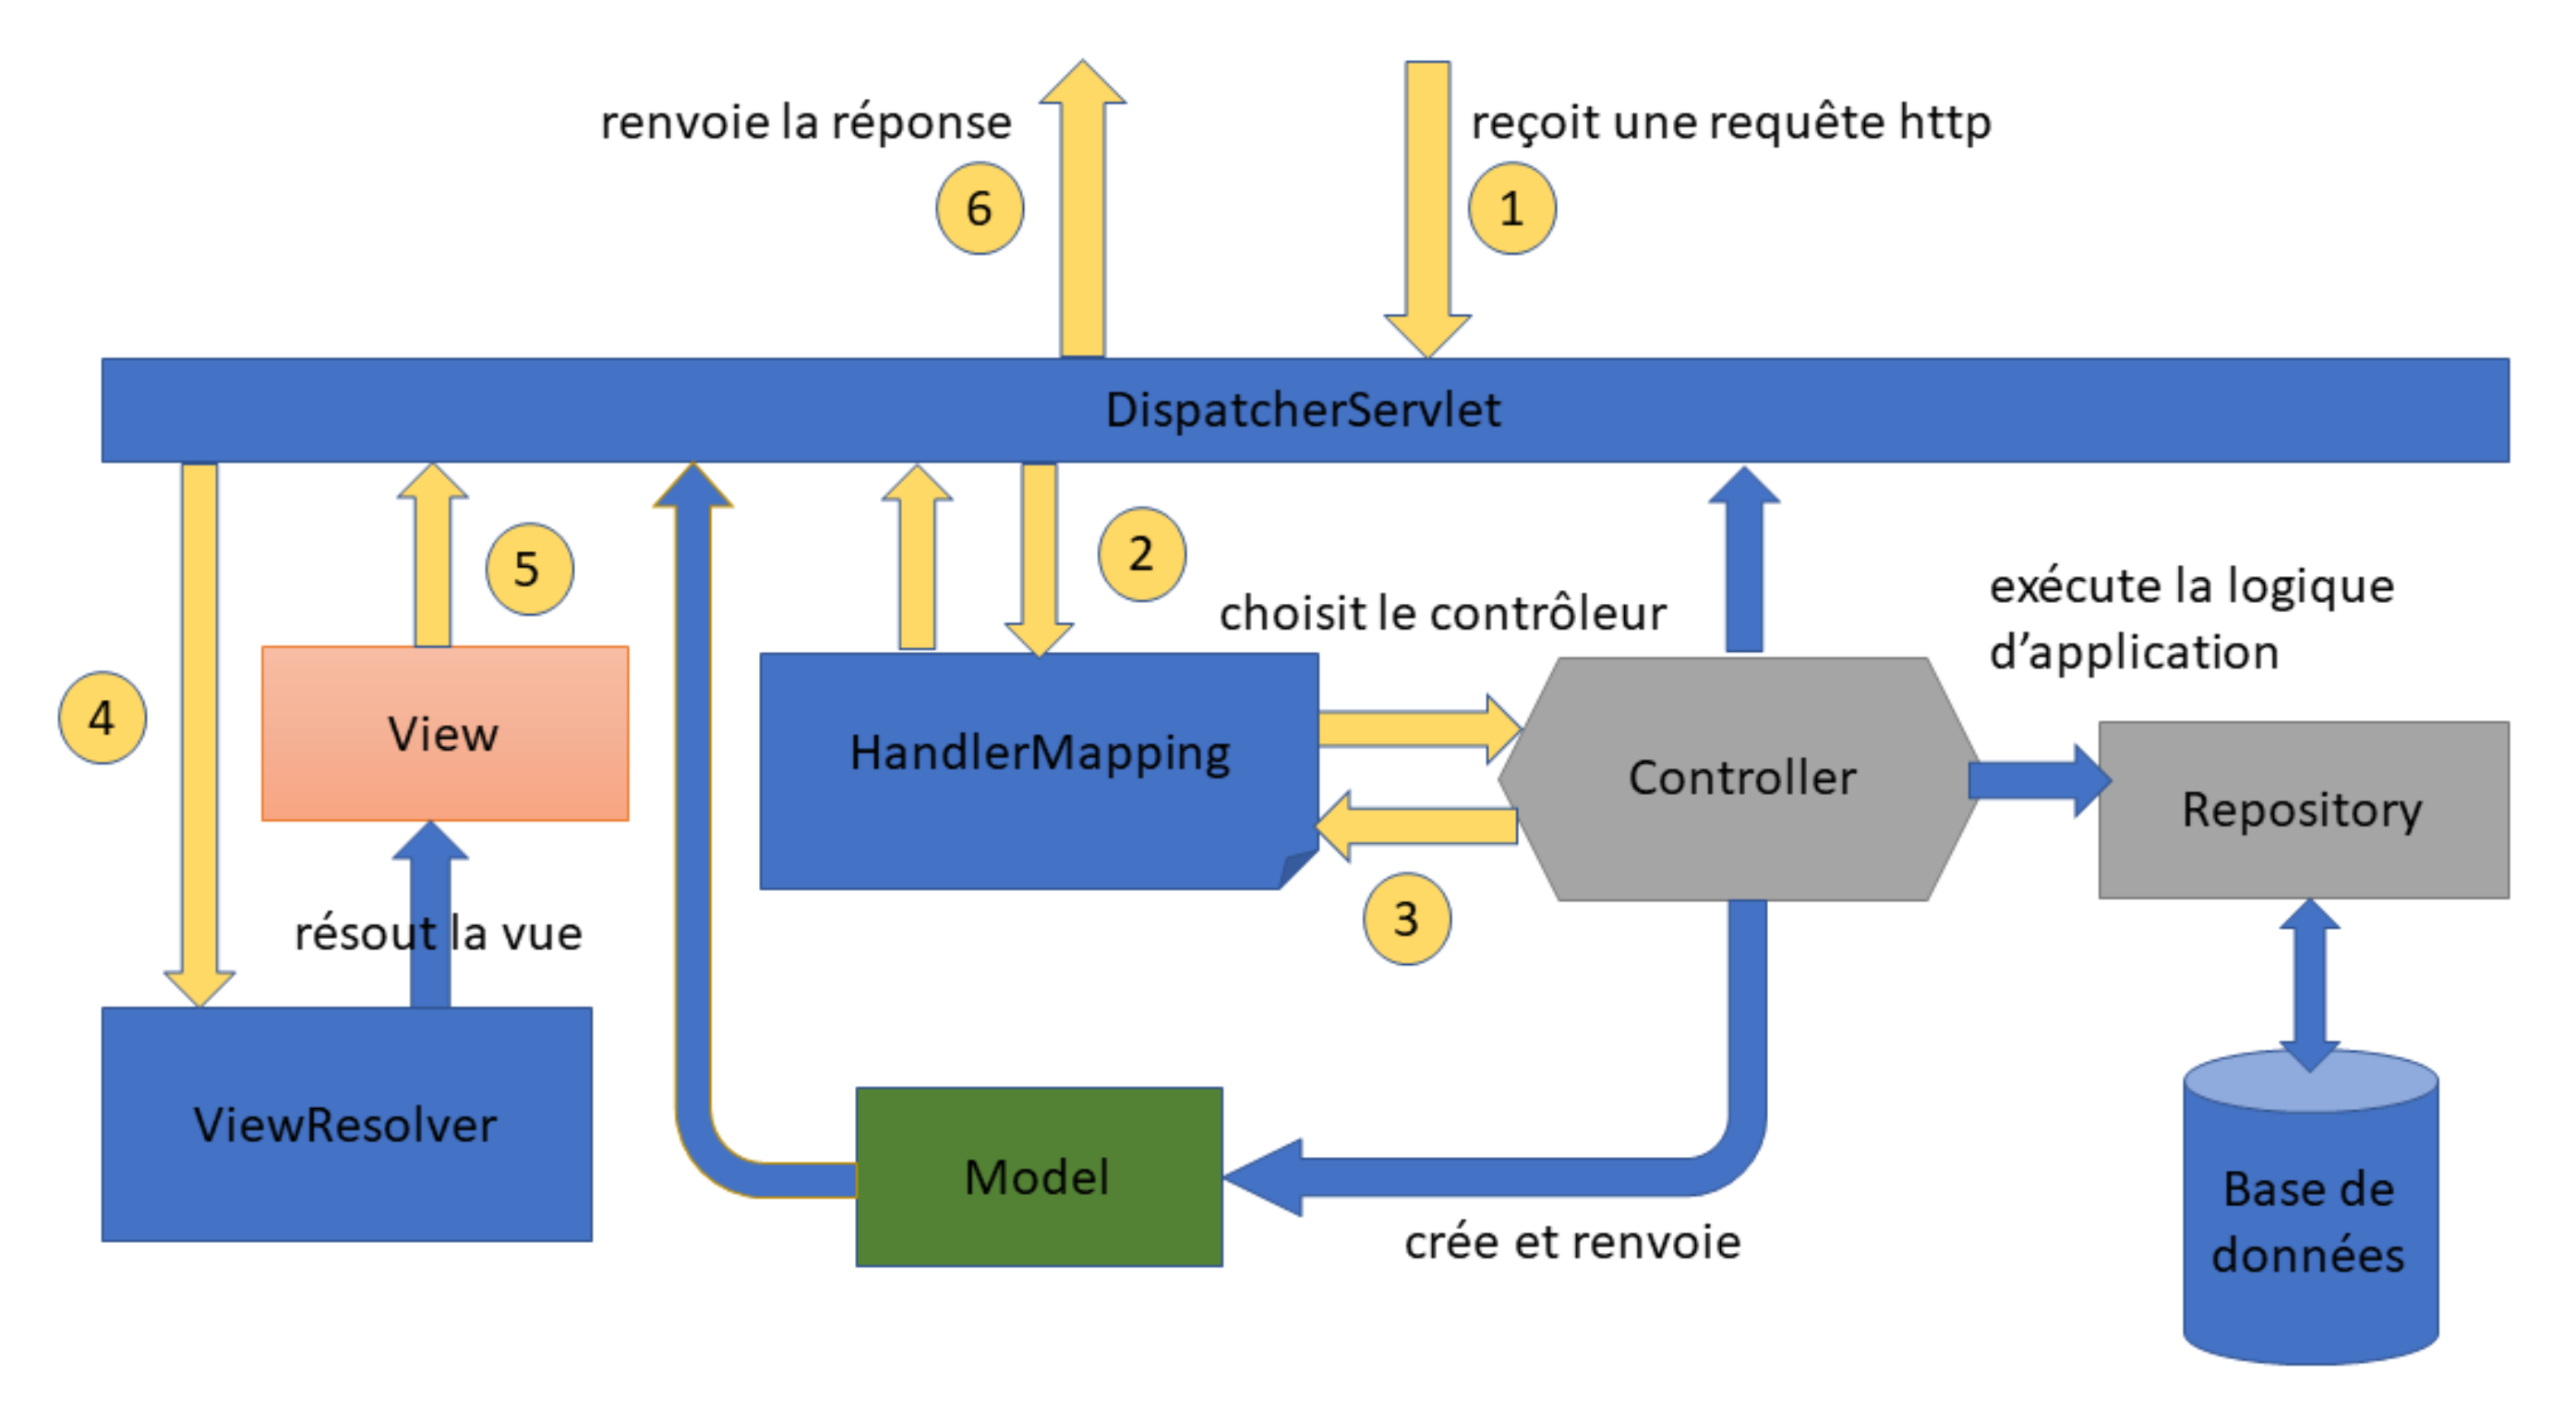
\includegraphics[width=1.0 \columnwidth]{figures/ArchitectureSpring.png}
    \caption{Architecture du framework \textit{Spring}}
    \label{fig:ArchitectureSpring}
\end{figure}

\textit{Spring Security} est une librairie du framework \textit{Spring} permettant la gestion de l’authentification et le contrôle d’accès. Comme le reste des projets Spring, il est facilement personnalisable. Son utilisation va permettre de faciliter l’utilisation du patron de sécurité avec PAMELA grâce à des classes relativement faciles à identifier. Nous allons pour cette expérimentation nous intéresser à l'authentification.

La figure \ref{fig:ArchitectureAuthentificationSpring} présente la gestion de l'authentification au sein du framework \textit{Spring}. Lorsque l’application développée avec \textit{Spring Security} reçoit une requête, la requête passe à travers une chaine de filtre (1) . Quand la requête contient une demande d’authentification, l’\textit{AuthenticationFilter} va extraire les informations d’identification de l’utilisateur (généralement son nom d’utilisateur et son mot de passe) et créer un objet \textit{Authentication}. Si les informations reçues contiennent un nom d’utilisateur et un mot de passe, un \textit{UsernamePasswordAuthenticationToken} sera créé contenant le nom d’utilisateur et le mot de passe (2) . Ce \textit{token} sera utilisé pour invoquer la méthode \textit{authenticate()} de l’\textit{AuthenticationManager} qui est implémenté par \textit{ProviderManager} (3) . Il existe plusieurs \textit{AuthenticationProvider} déjà configurés et listés dans \textit{ProviderManager}. Celui que nous utiliserons dans
cette expérimentation est le \textit{DAOAuthenticationProvider}. DAO correspond à "Data Access Object", c’est un modèle qui fournit une interface abstraite à un type de base de données. En mappant les appels d’application à la couche de persistance, le DAO fournit certaines opérations de données spécifiques sans exposer les détails de la base de données. Le \textit{DAOAuthenticationProvider} utilise \textit{UserDetailsService} (5) pour récupérer les données de l’utilisateur en fonction de son nom d’utilisateur (6) , (7) , (8) , (9) . Si l’authentification (10) réussit alors l’objet \textit{Authentication} complet (avec "authenticated = True", la liste des autorités et le nom d’utilisateur) est renvoyé. Sinon une exception \textit{AuthenticationException} sera levée. Enfin, \textit{AuthenticationManager} renvoie l’objet \textit{Authentication} à l’\textit{Authenticationfilter}, l’authentification a réussi et l’objet est stocké dans le \textit{SecurityContext}.

\begin{figure}[!h]
    \centering
    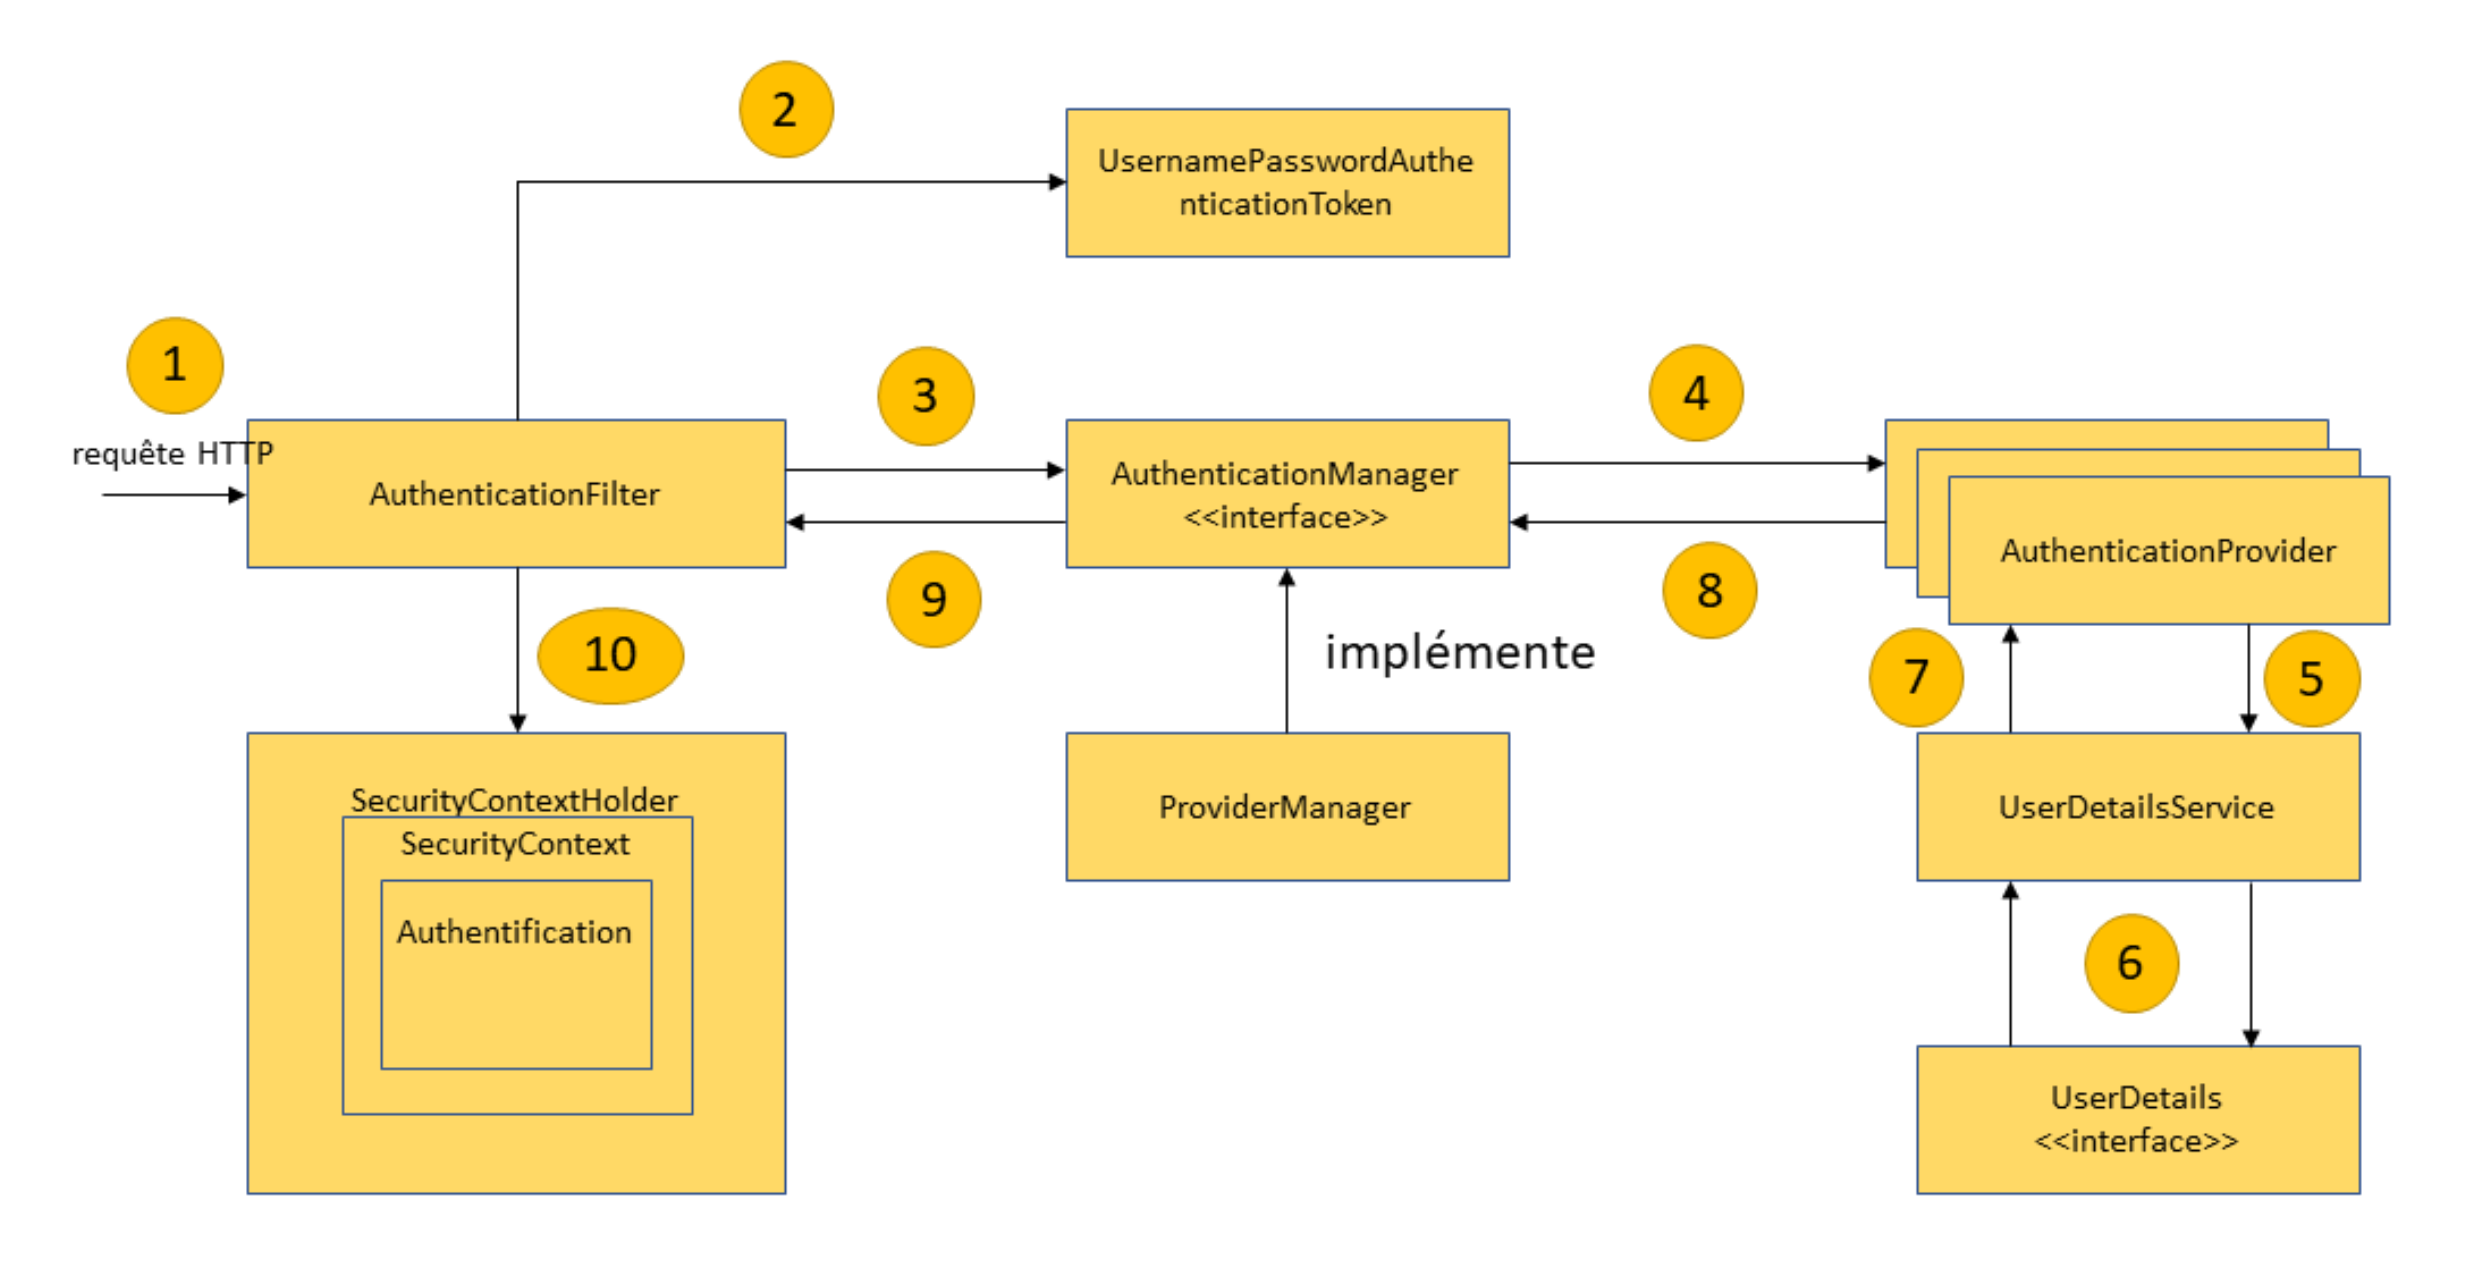
\includegraphics[width=1.0 \columnwidth]{figures/ArchitectureAuthentificationSpring.png}
    \caption{Gestion de l'authentification dans le framework \textit{Spring}}
    \label{fig:ArchitectureAuthentificationSpring}
\end{figure}

\subsection{Mise en oeuvre du patron \textit{Authenticator} sur une application Spring}

% PAMELA: un framework de tissage au run-time permettant de faire du monitoring de propriétés de sécurité

La mise en oeuvre du patron \textit{Authenticator} dans ce contexte s'appuie sur des techniques d'annotations de code source. Ces techniques requièrent d'identifier les concepts et les points d'extension adéquats, au prix parfois de la mise en place d'héritages et de délégations.

La figure \ref{fig:authenticator_class_diagram} reprend le diagramme de classe du patron \textit{Authenticator} présenté dans la section \ref{subsubsec:authenticator_pattern}. On se réfèrera également à la figure \ref{fig:AuthenticatorPattern} pour la correspondance des concepts entre les concepts métiers fournis par Spring et le patron \textit{Authenticator} utilisé.

Ce patron identifie quatre entités distinctes : \textit{Authenticator}, \textit{Subject}, \textit{AuthenticationInformation} et \textit{ProofOfIdentity}, pour lesquelles il s'agit de trouver le concept métier correspondant dans le code source à annoter.

\subsubsection{Authenticator} : Ce concept est identifié dans le patron \textit{Authenticator} avec l'annotation \texttt{@Authenticator}. Sur l'application à sécuriser, c'est l'API \textit{AuthenticationProvider} qui réalise cette fonctionnalité. Concrètement, nous allons utiliser la classe \textit{DAOAuthenticationProvider} (implantation d'une logique base de données avec accès à la couche donnée) qui prend en charge cette fonctionnalité. Nous avons ici choisi une logique d'héritage en définissant le couple API/implantation présenté dans le listing \ref{listing:CustomAuthenticationProvider}. L'identification du patron s'opère via l'identifiant \texttt{SessionInfo.PATTERN\_ID}, qui est une simple chaîne de caractères.

\begin{lstlisting}[language=Java,basicstyle=\ttfamily\footnotesize, caption=Mise en oeuvre de l'entité \textit{Authenticator} : \texttt{CustomAuthenticationProvider.java},label=listing:CustomAuthenticationProvider]
@ModelEntity
@ImplementationClass(CustomAuthenticationProviderImpl.class)
@Authenticator(patternID = SessionInfo.PATTERN_ID)
@Imports(@Import(SessionInfo.class))
public interface CustomAuthenticationProvider extends AuthenticationProvider {
  String USER_NAME = "userName";

  // Inherited from AuthenticationProvider API
  public Authentication authenticate(Authentication authentication) throws AuthenticationException;

    ...

  // This method retrieve proof of identity given supplied authentication information
  @RequestAuthentication(patternID = SessionInfo.PATTERN_ID)
  UsernamePasswordAuthenticationToken request(
    @AuthenticationInformation(
      patternID = SessionInfo.PATTERN_ID, 
      paramID = USER_NAME) 
    String userName);

  abstract class CustomAuthenticationProviderImpl extends DaoAuthenticationProvider implements CustomAuthenticationProvider {

    @Override
    public Authentication authenticate(Authentication authentication) throws AuthenticationException {
      ...
    }

    @Override
    public UsernamePasswordAuthenticationToken request(String userName) {
      ...
    }
  }
}
\end{lstlisting}

\subsubsection{Subject} : Ce concept est identifié dans le patron \textit{Authenticator} avec l'annotation \texttt{@AuthenticatorSubject}. Sur l'application à sécuriser, ce concept correspond peu ou prou à la notion de session, mais n'est pas directement réifé. Nous choisissons de le faire en déclarant le couple API/implantation \texttt{SessionInfo}, présenté dans le listing suivant (nous présenterons plus loin la gestion du cycle de vie de cette donnée):

\begin{lstlisting}[language=Java,basicstyle=\ttfamily\footnotesize, caption=Mise en oeuvre de l'entité \textit{Subject} : \texttt{SessionInfo.java},label=listing:SessionInfo]
@ModelEntity
@ImplementationClass(SessionInfo.SessionInfoImpl.class)
@AuthenticatorSubject(patternID = SessionInfo.PATTERN_ID)
public interface SessionInfo {

	String SESSION_INFO = "SESSION_INFO";
	String PATTERN_ID = "AuthenticatorPattern";
	String USER_NAME = "username";
	String IP_ADRESS = "ipAdress";
	String AUTHENTICATION_PROVIDER = "authenticationProvider";
	String ID_PROOF = "idProof";

	@Getter(USER_NAME)
	@AuthenticationInformation(patternID = PATTERN_ID, paramID = CustomAuthenticationProvider.USER_NAME)
	String getUserName();

	@Setter(USER_NAME)
	void setUserName(String val);
	
	@Setter(IP_ADRESS)
	void setIpAdress(String val);
	
	@Getter(IP_ADRESS)
	String getIpAdress();

	@Getter(value = ID_PROOF, ignoreType = true)
    UsernamePasswordAuthenticationToken getIDProof();

	@Setter(ID_PROOF)
	@ProofOfIdentitySetter(patternID = PATTERN_ID)
	void setIdProof(UsernamePasswordAuthenticationToken value);

	@Getter(AUTHENTICATION_PROVIDER)
	@AuthenticatorGetter(patternID = PATTERN_ID)
	CustomAuthenticationProvider getAuthenticationProvider();

	@Setter(AUTHENTICATION_PROVIDER)
	void setAuthenticationProvider(CustomAuthenticationProvider val);

	@AuthenticateMethod(patternID = PATTERN_ID)
	void authenticate();

    /**
      * Ensure call-stack is executed in authenticated context relatively 
      * to this {@link SessionInfo} (because this method is annotated with 
      * @RequiresAuthentication, calling it MUST be performed in
      * authenticated context)
      */
	@RequiresAuthentication
	void checkSecure();

	abstract class SessionInfoImpl implements SessionInfo {

        ...
        
		@Override
		public void checkSecure() {
			System.out.println("checkSecure() for " + this);
		}

		@Override
		public String getIpAdress() {
			return ((ServletRequestAttributes)RequestContextHolder.currentRequestAttributes())
			           .getRequest().getRemoteAddr();
		}
	}

}
\end{lstlisting}

La notion de session (\textit{SessionInfo}) (listing \ref{listing:SessionInfo}) permet la gestion du \texttt{USER\_NAME}, \texttt{IP\_ADDRESS} et \texttt{ID\_PROOF} (preuve d'identité), ainsi que l'accès à l'authenticator via les accesseurs \texttt{getAuthenticationProvider()} et \texttt{setAuthenticationProvider(CustomAuthenticationProvider)}

La méthode \texttt{authenticate()} (ligne 41 du listing \ref{listing:SessionInfo}) est identifiée via l'annotation \texttt{@AuthenticateMethod} qui indique que cette méthode correspond à la requête d'identification du patron \textit{Authenticator} comme présenté dans la figure \ref{fig:AuthenticatorPattern}.

\subsubsection{AuthenticationInformation} : L'information à la base de l'authentification dans l'application Spring à sécuriser est le nom utilisateur défini dans la classe \textit{SessionInfo} (listing \ref{listing:SessionInfo}). Il s'agit d'une simple chaîne de caractères définie à partir des accesseurs \texttt{getUserName()} et \texttt{setUserName(String)} définis respectivement lignes 15 et 18 du listing  \ref{listing:SessionInfo}. L'annotation \texttt{@AuthenticationInformation} définie ligne 14 précise l'utilisation de cette donnée pour l'authentification, conjointement avec l'annotation \texttt{@AuthenticationInformation(paramId=...)} définie ligne 14 du listing \ref{listing:CustomAuthenticationProvider}.

\subsubsection{ProofOfIdentity} : La quatrième et dernière entité à identifier est la notion de preuve d'identité que l'on retrouve dans la classe \texttt{UsernamePasswordAuthenticationToken} dans l'application Spring à sécuriser. Nous avons choisi d'exposer le couple d'accesseurs getIDProof() et setIDProof(UsernamePasswordAuthenticationToken) dans l'interface SessionInfo (respectivement lignes 27 et 31 du listing \ref{listing:SessionInfo}.

\subsubsection{Cycle de vie de la notion d'\texttt{AuthenticationProvider}} :

Nous avons utilisé la notion de \textit{Service} offerte par le framework Spring pour implanter un service dédié à l'authentification. Le listing \ref{listing:AuthManagerService} présente cette implantation. C'est ce service qui sera responsable de l'instantiation d'une unique instance (singleton) de \texttt{CustomAuthenticationProvider} pour l'application et de la création de session (\texttt{SessionInfo}), via l'utilisation d'une factory basée sur la construction du \texttt{PamelaMetaModel} inféré à partir de la classe \texttt{CustomAuthenticationProvider} (lignes 11 et 12 du listing \ref{listing:AuthManagerService}). Ce même service gère également avec la même factory l'instantiation d'une instance de \texttt{SessionInfo}.

\begin{lstlisting}[language=Java,basicstyle=\ttfamily\footnotesize, caption=Mise en oeuvre du service d'authentification : \texttt{AuthManagerService.java},label=listing:AuthManagerService]
@Service
public class AuthManagerService {

	private CustomAuthenticationProvider authenticationProvider;

	private PamelaModelFactory factory;

	public AuthManagerService() {
		PamelaMetaModel pamelaMetaModel;
		try {
			pamelaMetaModel = new PamelaMetaModel(CustomAuthenticationProvider.class);
			factory = new PamelaModelFactory(pamelaMetaModel);
		} catch (ModelDefinitionException e) {
			e.printStackTrace();
		}

		authenticationProvider = factory.newInstance(CustomAuthenticationProvider.class);
	}

	public CustomAuthenticationProvider getAuthenticationProvider() {
		return authenticationProvider;
	}

	public SessionInfo makeNewSessionInfo() {
		SessionInfo returned = factory.newInstance(SessionInfo.class);
		returned.setAuthenticationProvider(getAuthenticationProvider());
		return returned;
	}
}
\end{lstlisting}

\subsubsection{Cycle de vie de la notion de session (SessionInfo)} : 

Nous avons utilisé le composant Spring \texttt{HttpSessionEventPublisher} comme support de points d'extension permettant de gérer la construction et la destruction d'instances de \texttt{SessionInfo}. Nous proposons dans le listing \ref{listing:CustomHttpSessionEventPublisher} une classe \texttt{CustomHttpSessionEventPublisher} qui hérite de \texttt{HttpSessionEventPublisher} et qui implante ces fonctionnalités de gestion d'instances de \texttt{SessionInfo} (lignes 12 et 21 respectivement pour la création et la destruction d'instances).

\begin{lstlisting}[language=Java,basicstyle=\ttfamily\footnotesize, caption=Cycle de vie des \texttt{SessionInfo} : \texttt{CustomHttpSessionEventPublisher.java},label=listing:CustomHttpSessionEventPublisher]
@Component
public class CustomHttpSessionEventPublisher 
extends HttpSessionEventPublisher {

	@Autowired
	private AuthManagerService authManagerService;

	@Override
	public void sessionCreated(HttpSessionEvent event) {
		super.sessionCreated(event);
		if (event.getSession().getAttribute(SessionInfo.SESSION_INFO) == null) {
			SessionInfo sessionInfo = authManagerService.makeNewSessionInfo();
			event.getSession().setAttribute(SessionInfo.SESSION_INFO, sessionInfo);
		}
	}

	@Override
	public void sessionDestroyed(HttpSessionEvent event) {
		super.sessionDestroyed(event);
		// delete the session
    ((SessionInfo)event.getSession().getAttribute(SessionInfo.SESSION_INFO)).delete();
	}
}
\end{lstlisting}

\subsubsection{Gestion de l'authentification} : 

La gestion de l'authentification proprement dite est rendue délicate du fait de deux paradigmes concurrents pour l'authentification: celui fourni par le framework Spring et celui implanté dans le patron \textit{Authenticator}. L'alignement des deux mécanismes s'opère dans l'implantation de \texttt{CustomAuthenticationProviderImpl} (listing \ref{listing:CustomAuthenticationProviderImpl}). C'est le framework Spring qui reçoit les requêtes d'authentification via l'appel de la méthode \texttt{authenticate(Authentication)} de \texttt{AuthenticationProvider}. Nous avons surchargé cette méthode avec la gestion de la \texttt{SessionInfo} courante, mais surtout en remplissant une table de correspondance entre le nom utilisateur servant d'information d'authentification et la preuve d'identité retournée par le \texttt{AuthenticationProvider} (une instance de \texttt{UsernamePasswordAuthenticationToken}). L'implantation de la méthode \texttt{request(String)} est alors triviale en ce sens qu'il suffit de retourner cette même valeur.

\begin{lstlisting}[language=Java,basicstyle=\ttfamily\footnotesize, caption=Gestion de l'authentification : détail de \texttt{CustomAuthenticationProvider.java},label=listing:CustomAuthenticationProviderImpl]
abstract class CustomAuthenticationProviderImpl extends DaoAuthenticationProvider implements CustomAuthenticationProvider {

    private Map<String, UsernamePasswordAuthenticationToken> tokens 
        = new HashMap<>();
        
	/**
      * Implementation is here trivial as we use map filled by
      * {@link #authenticate(Authentication)} method
		 */
	@Override
	public UsernamePasswordAuthenticationToken request(String userName) {
		return tokens.get(userName);
	}

	@Override
	public Authentication authenticate(Authentication authentication) throws AuthenticationException {

		try {
			System.out.println("authenticate(Authentication) called for " + authentication);
			UsernamePasswordAuthenticationToken returned = (UsernamePasswordAuthenticationToken) super.authenticate(authentication);
			String name = authentication.getName();
			WebAuthenticationDetails details = (WebAuthenticationDetails) authentication.getDetails();
			String userIp = details.getRemoteAddress();
			SessionInfo sessionInfo = SessionInfo.getCurrentSessionInfo();
			sessionInfo.setUserName(name);
			sessionInfo.setIpAdress(userIp);
			tokens.put(name, returned);
			// Call authenticate() to complete process
			sessionInfo.authenticate();
			// Ensure that we are now in authenticated context
			sessionInfo.checkSecure();
			return returned;
		} catch (AuthenticationException e) {
			throw e;
		} catch (ModelExecutionException e) {
			e.printStackTrace();
			throw new SessionAuthenticationException("Exception during authentication: " + e.getMessage());
        }

	}
}
\end{lstlisting}

\subsection{Expérimentation de l'application sécurisée}

La mise en oeuvre du patron \textit{Authenticator} sur l'application sécurisée est relativement transparente pour l'utilisateur, d'un point de vue fonctionnel. Cependant le mécanisme de tissage au run-time gère maintenant explicitement des instances du patron  \textit{Authenticator} (\textit{AuthenticatorPatternInstance}), avec leur propre cycle de vie qui évolue au fur et à mesure des créations et suppressions de sessions dans l'application web. La classe \textit{SessionInfo} est dorénavant dotée d'un mode authentifié, dans la mesure où les méthodes annotées avec \textit{@RequiresAuthentication} (ex: méthode \texttt{checkSecure()}, ligne 50 du listing \ref{listing:SessionInfo}) ne peuvent s'exécuter que si l'instance courante est bien déclarée comme sujet d'une instance du patron \textit{Authenticator} pour laquelle l'authentification a été satisfaite. Ceci permet de protéger tout appel de code non autorisé et malveillant dans le contexte d'une vulnérabilité qui donnerait accès à l'exécution de ce code.

Le patron \textit{Authenticator} définit intrinsèquement 6 propriétés (4 propriétés implicites et deux propriétés fonctionnelle), qui ont été décrites dans la section \ref{subsubsec:AuthenticatorCyberContract}. La mise en oeuvre du patron garantit donc sur l'application sécurisée la vérification au run-time (monitoring) de l'ensemble de ces six propriétés, et ce dans le cadre de tous les appels aux méthodes des instances des classes concernées par le patron (ici \textit{SessionInfo} et \textit{CustomAuthenticationProvider}). 

\begin{enumerate}
    \item \textbf{Unicité du couple sujet/informations d'authentification}
    \begin{equation*}
        P1: \forall a, b \in I_{Subject}, a \ne b \implies a.authInfo \ne b.authInfo
    \end{equation*}
    Sur l'application déployée, cette première propriété se traduit par l'impossible pour un même nom d'utilisateur d'être utilisé dans deux sessions différentes: si un utilisateur est loggué, il lui faut d'abord se délogguer avant de pouvoir ouvrir une autre session. L'expérimentation peut se faire sur deux navigateurs différents: l'ouverture d'une deuxième session déclenche une exception \texttt{ModelExecutionException} (\textit{Subject Invariant Violation: Authentication information are not unique}). 
    \\
    \item \textbf{Non usurpation des informations d'authentification}
    \begin{equation*}
        P2: \forall a \in I_{Subject}, a.authInfo = a.authInfo_{ini}
    \end{equation*}
    Cette propriété garantit la non-usurpation des informations d'authentification. Concrètement, la propriété \texttt{userName} de \texttt{SessionInfo} ne pourra être modifiée durant toute la durée de vie de l'instance de \texttt{SessionInfo}, sans déclencher une exception \texttt{ModelExecutionException} (\textit{Subject Invariant Violation: Authentication Information has changed since initialization}). 
    \\
    \item \textbf{Intégrité de l'autorité d'authentification}
    \begin{equation*}
        P3: \forall a \in I_{Subject}, a.authenticator = a.authenticator_{ini}
    \end{equation*}
    Si un attaquant réussi à forger son \textit{Authenticator} il devient maître du système d'authentification. Il est donc essentiel que l'\textit{Authenticator} ne puisse pas être modifié, ce que garantit cette propriété.
    \\
    \item \textbf{Vérification continue d'une preuve d'identité valide ou indéfinie}
    \begin{equation*}
      \begin{split}
        &P4: \forall a \in I_{Subject}, (a.idProof = \emptyset) \lor \\&(a.idProof = a.authenticator.request(a.authInfo))
      \end{split}
    \end{equation*}
    A tout moment, la preuve d’identité de chaque sujet doit être soit valide, soit non définie. 
    \\
    \item \textbf{Vérification continue de la preuve d'identité}
    \begin{equation*}
        P5: self.idProof = self.authenticator.request(self.authInfo)
    \end{equation*}
    Après l'authentification, la preuve d'identité doit toujours correspondre à la valeur renvoyée par la méthode de requête avec les bons paramètres. La vérification conjointe des propriétés P4 et P5 garantit pendant toute la durée de la session la validité de la preuve d'identité et prévient une éventuelle attaque par \textit{"pivoting"}.
    \\
    \item \textbf{Post-condition de la méthode \textit{request(authInfo)}}
    \begin{equation*}
        P6: self.check(authInfo) \lor returnValue = \emptyset
    \end{equation*}
    La preuve d'identité renvoyée par la méthode \textit{request(authInfo)} de la classe \textit{Authenticator} doit être valide si et seulement si le sujet qui la demande est bien celui qu'il prétend être. La vérification de cette propriété garantit cette assertion. 
 \end{enumerate}

\subsection{Configuration du monitoring}
\label{subsec:conf-monitoring}

\sg{Proposition : mettre ca plutot dans la discussion plus loin}

A noter que la portée du monitoring est configurable via l'annotation \texttt{@MonitoredEntity} qui définit cinq stratégies possibles :
\begin{itemize}
    \item Vérification à l'entrée et à la sortie (ou à la sortie seulement) de toutes les méthodes, sauf les méthodes internes
    \item Vérification à l'entrée et à la sortie (ou à la sortie seulement) de toutes les méthodes sauf celles déclarées explicitement comme non-monitorées
    \item Vérification à l'entrée et à la sortie (ou à la sortie seulement) de toutes les méthodes coucourant à l'exécution du patron et des méthodes déclarées explicitement comme monitorées
    \item Vérification à l'entrée et à la sortie (ou à la sortie seulement) de toutes les méthodes déclarées explicitement comme monitorées
    \item Pas de vérification (pas de monitoring)
\end{itemize}
Il est également possible d'activer ou de désactiver le monitoring , et d'augmenter ou de diminuer le niveau de monitoring de façon programmatique.

\subsection{Spécialisation du patron \textit{Authenticator} et ajout d'une propriété de sécurité exprimée en logique temporelle}

La réification de la notion d'instance de patron \textit{Authenticator} (au travers ici d'une instance de la classe \texttt{AuthenticatorPatternInstance}, liée aux instances de sujet (classe \texttt{SessionInfo}) et d'authenticator (classe \texttt{CustomAuthenticationProvider}), et dont l'exécution est tissée au run-time) présente l'avantage de la gestion d'un état, et donc de l'exécution de code métier lié à l'assemblage de ces classes.

Un deuxième intérêt de cette approche réside dans la capacité du framework à étendre l'implantation standard du patron \textit{Authenticator}.

Nous avons mis à profit ces deux aspects pour spécialiser le patron \textit{Authenticator} et implanter une nouvelle propriété à la fois liée à la logique temporelle et également temporisée. Cette propriété exprime le fait qu'il ne peut pas y avoir plus de trois échecs d'authentification dans un labs de temps déterminé. Si trois échecs arrivent dans ce temps, l'application devra passer dans un autre mode (refusant toute tentative d'authentification pendant un certain temps par exemple).

Soit $auth\_fail_i$ un évènement "échec d'authentification" dans la trace d'exécution courante \textit{execution\_trace} :

    \begin{equation*}
       \begin{split}
           P7:& \forall \{ auth\_fail_i,auth\_fail_{i+1},auth\_fail_{i+2} \} \in execution\_trace \\
          &auth\_fail_{i+2}.time - auth\_fail_i.time < TIME\_LIMIT
      \end{split}
    \end{equation*}

La spécialisation du patron \textit{Authenticator} requiert la définition des trois classes présentées dans les listings \ref{listing:CustomAuthenticatorPatternFactory}, \ref{listing:CustomAuthenticatorPatternDefinition} et \ref{listing:CustomAuthenticatorPatternInstance}. La classe \texttt{CustomAuthenticatorPatternInstance} implante concrètement la définition de la propriété \textit{P7} tandis que le listing \ref{listing:TemporalPropertyDefinition} complète la définition de l'\textit{authenticator} \texttt{CustomAuthenticationProvider} en faisant référence à cette propriété comme précondition de la méthode \texttt{authenticate(Authentication)} (ligne 6). A noter également ligne 9 l'utilisation de l'annotation \texttt{@OnException} qui permet de gérer automatiquement la génération d'évènements correspondant à l'échec de connexion, dont la trace est accessible à l'instance courante.



\begin{lstlisting}[language=Java,basicstyle=\ttfamily\footnotesize, caption=Spécialisation de la classe \texttt{AuthenticatorPatternFactory.java},label=listing:CustomAuthenticatorPatternFactory]
public class CustomAuthenticatorPatternFactory extends AuthenticatorPatternFactory {

	public CustomAuthenticatorPatternFactory(PamelaMetaModel metaModel) {
		super(metaModel);
	}

	@Override
	protected Class<CustomAuthenticatorPatternDefinition> getPatternDefinitionClass() {
		return CustomAuthenticatorPatternDefinition.class;
	}

	@Override
	protected CustomAuthenticatorPatternDefinition getPatternDefinition(String patternId, boolean createWhenNonExistant) {
		return (CustomAuthenticatorPatternDefinition) super.getPatternDefinition(patternId, createWhenNonExistant);
	}
}
\end{lstlisting}

\begin{lstlisting}[language=Java,basicstyle=\ttfamily\footnotesize, caption=Spécialisation de la classe \texttt{AuthenticatorPatternDefinition.java},label=listing:CustomAuthenticatorPatternDefinition]
public class CustomAuthenticatorPatternDefinition extends AuthenticatorPatternDefinition {

	public CustomAuthenticatorPatternDefinition(String identifier, PamelaMetaModel pamelaMetaModel) {
		super(identifier, pamelaMetaModel);
	}

	@Override
	public <I> void notifiedNewInstance(I newInstance, ModelEntity<I> modelEntity, PamelaModel model) {
		if (modelEntity == getSubjectModelEntity()) {
			// We create a new PatternInstance for each new instance of subjectModelEntity
			CustomAuthenticatorPatternInstance<?, I, ?, ?> newPatternInstance = new CustomAuthenticatorPatternInstance(this, model,
					newInstance);
		}
	}
}
\end{lstlisting}

\begin{lstlisting}[language=Java,basicstyle=\ttfamily\footnotesize, caption=Spécialisation de la classe \texttt{AuthenticatorPatternInstance.java},label=listing:CustomAuthenticatorPatternInstance]
public class CustomAuthenticatorPatternInstance extends AuthenticatorPatternInstance<CustomAuthenticationProvider, SessionInfo, String, UsernamePasswordAuthenticationToken> {

	public CustomAuthenticatorPatternInstance(CustomAuthenticatorPatternDefinition patternDefinition, PamelaModel model, SessionInfo subject) {
		super(patternDefinition, model, subject);
	}

	public void checkAuthFailCount() {
		// Perform check that last 3 AuthFailEvent in current execution trace were not raised within allowed time limit
        ...
	}
\end{lstlisting}

\begin{lstlisting}[language=Java,basicstyle=\ttfamily\footnotesize, caption=Définition de la propriété temporelle,label=listing:TemporalPropertyDefinition]
public interface CustomAuthenticationProvider extends AuthenticationProvider {

    ...
    
	@Override
	@Requires(
			patternID = SessionInfo.PATTERN_ID,
			property = "patternInstance.checkAuthFailCount()")
	@OnException(exceptionClass = AuthenticationException.class, generateEvent = AuthFailEvent.class)
    public Authentication authenticate(Authentication authentication) throws AuthenticationException;

    ...
}
\end{lstlisting}

Tout appel de la méthode \texttt{authenticate(Authentication)} est dorénavant surveillé par l'instance \texttt{CustomAuthenticatorPatternInstance} correspondante, qui gère automatiquement les évènements \texttt{AuthFailedEvent}, et qui vérifie qu'un utilisateur ne peut pas échouer à s'authentifier plus de 3 fois dans un temps donné. 

Cette expérimentation montre comment il est possible d'étendre le patron \textit{Authenticator} pour faire en sorte de vérifier à la fois les propriétés P1-P6 définies pour ce patron, ainsi que d'autres propriétés plus spécialisées (P7).


